Owing to the principles of quantum superposition, quantum entanglement, and quantum parallelism, quantum algorithms have the capacity to efficiently address certain computational problems, such as Shor's algorithm \cite{shor1994algorithms}, Grover's algorithm \cite{grover1996fast,long2001grover} and Harrow-Hassidim-Lloyd algorithm \cite{harrow2009quantum}, achieving exponential or polynomial acceleration when compared to classical algorithms. Nevertheless, the current stage of quantum devices is constrained by limited quantum qubits and significant noise, which is often referred to as Noisy Intermediate-Scale Quantum (NISQ) devices \cite{preskill2018quantum}. It is worth noting that the quantum algorithms mentioned above do not exhibit quantum advantage under NISQ era.

Variational Quantum Algorithms (VQA) \cite{cerezo2021variational,yuan2019theory,xu2021variational} are considered the most promising candidates for achieving quantum advantage in the NISQ era. VQA leverages optimization algorithms from classical machine learning to fine-tune parameterized quantum circuits (PQC). As a result, VQA is a hybrid quantum-classical algorithm. VQA has found extensive applications in various domains, including quantum many body simulations \cite{Peruzzo2014Peruzzo2014,kandala2017hardware,kokail2019self,lyu2023variational,Lyu2023symmetryenhanced,cao2022progress}, quantum approximate optimization algorithm \cite{farhi2014quantum,patti2022variational,chandarana2023digitized}, quantum machine learning \cite{benedetti2019parameterized,wei2022quantum,lloyd2018quantum,biamonte2017quantum,abbas2021power} and entanglement purification \cite{zhang2023variational}. In this section, we will provide a brief overview of the VQA algorithm's workflow and how it can be efficiently implemented in \MindQuantum. More examples of VQA algorithm applications will be present in chapter \ref{sec:applications}.

\begin{figure}[h]
  \begin{center}
    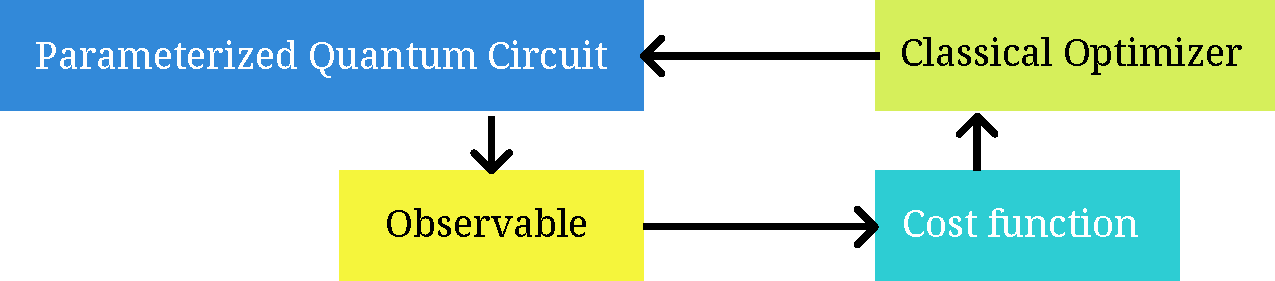
\includegraphics[width=0.9\linewidth]{images/4_1_vqa.pdf}
  \end{center}
  \caption{The work flow of VQA.}
  \label{fig:vqa_work_flow}
\end{figure}

Fig.~\ref{fig:vqa_work_flow} illustrates the primary workflow of the VQA. The central component of VQA is the PQC, which comprises both non-parameterized gates such as Hadamard and Pauli gates, and parameterized gates like the rotation gates around the $x$, $y$, or $z$ axes of the Bloch sphere. Depending on the specific task, the PQC can be divided into two parts: the encoder circuit, responsible for encoding classical data into a quantum state denoted as $U_e(\alpha)$, and the ansatz circuit, serving as the trainable component of VQA, denoted as $U_a(\theta)$.

In VQA, we also require an observable operator denoted as $H$. The expectation value of this observable is calculated as follows:

\begin{equation}
  E(\alpha, \theta) = \bra{0}U_e^\dagger(\alpha)U_a^\dagger(\theta)HU_a(\theta)U_e(\alpha)\ket{0}.
\end{equation}
In quantum many-body simulation and quantum approximate optimization algorithm, we need to convert the problem into an observable and optimize the parameter $\theta$ to find the ground state of this observable (the encoder circuit $U_e$ is always identity in these problems). The task is described as:

\begin{equation}
  \min_\theta E(\theta).
\end{equation}
On the other hand, we need to define a cost function when we treat VQA as a part of machine learning model:

\begin{equation}
  \min_\theta L(E(\alpha, \theta), E_\text{target}),
\end{equation}
where $E_\text{target}$ is the target of the training model and $L$ is a cost function like mean absolute error loss or mean squared error loss.

Optimization algorithms in VQA can be categorized into two types based on their reliance on gradients. The first category comprises gradient-based optimization algorithms such as Adam and BFGS. These algorithms are well-suited for implementation in quantum simulators. The second category consists of non-gradient optimization algorithms such as SPSA and Nelder-Mead. These algorithms find more practical utility in real-world quantum experiments. In \MindQuantum, we are always focusing on gradient based optimizer, and we will show more detail about how we speed up the calculation of gradient of PQC in section \ref{sec:benchmark}.

\subsubsection{Learning a rotation}

In this subsection, we will delve into the implementation of variational quantum algorithms in \MindQuantum\ by exploring a task of learning a rotation quantum gate.

Suppose we have an initial quantum state $\ket{\psi_0}=\ket{0}$, and we are going to find a single qubit unitary operator $U(\theta)$, which can rotate $\ket{\psi_0}$ to $\ket{\psi_f}$ so that to minimum $E_X(\theta) = \bra{\psi_f}X\ket{\psi_f}$:

\begin{equation}
  \min_\theta(\bra{0}U^\dagger(\theta)XU(\theta)\ket{0}).
\end{equation}

The first step of VQA is to build an ansatz. In this task, we choose arbitrary single qubit rotation gate \Uthree to work as ansatz and \Uthree can also decompose into:

\begin{equation}
  U_3(a, b, c) = RZ(b)RX(-\pi/2)RZ(a)RX(\pi/2)RZ(c).
\end{equation}

\begin{lstlisting}
import numpy as np
from mindquantum.core.circuit import Circuit

ansatz = Circuit().rz('c', 0).rx(np.pi/2, 0)
ansatz.rz('a', 0).rx(-np.pi/2, 0).rz('b', 0)
ansatz.svg()
\end{lstlisting}

\begin{figure}[h]
  \begin{center}
    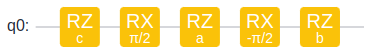
\includegraphics[width=0.9\linewidth]{images/4_1_ansatz.png}
  \end{center}
  \caption{The ansatz circuit that can be work as an arbitrary single qubit rotation.}
  \label{fig:u3_ansatz}
\end{figure}

The observable is implemented as:

\begin{lstlisting}
from mindquantum.core.operators import QubitOperator
from mindquantum.core.operators import Hamiltonian

obs = QubitOperator('X0')
ham = Hamiltonian(obs)
\end{lstlisting}

In \MindQuantum, the simulator provide a method \getexpectationwithgrad to easily calculate the gradient of $E_X(\theta)$.

\begin{lstlisting}
import numpy as np
from mindquantum.simulator import Simulator

sim = Simulator('mqvector', ansatz.n_qubits)
grad_ops = sim.get_expectation_with_grad(ham, ansatz)

p0 = np.random.uniform(-np.pi, np.pi, len(ansatz.params_name))
f, g = grad_ops(p0)
print(f, g)
\end{lstlisting}
And the output is:
\begin{lstlisting}
[[-0.04602095+0.j]] [[[-1.17340357e-17+0.j -3.47310364e-02+0.j -7.96875999e-01+0.j]]]
\end{lstlisting}

\getexpectationwithgrad receives observable Hamiltonian and ansatz circuit and returns a gradient operator. You can use this operator to calculate gradient in any ansatz parameters. The output of gradient operator is the expectation and its gradient with respect to ansatz parameters. The dimension of expectation value is $[n_\text{batch}, n_\text{ham}]$, where $n_\text{batch}$ is the batch size of encoder data and $n_\text{ham}$ is the number of Hamiltonian. In this task, we do not have encoder and we have only one observable, so $n_\text{batch}=1, n_\text{ham}=1$. The dimension of gradient of ansatz is $[n_\text{batch}, n_\text{ham}, n_\text{ansatz}]$, while $n_\text{ansatz} = 3$ is the number of parameters in ansatz circuit.

The next step is to optimize the PQC with the help of gradient operator.
\begin{lstlisting}
from scipy.optimize import minimize

def fun(p0, grad):
  f, g = grad(p0)
  f = np.real(f)[0, 0]
  g = np.real(g)[0, 0]
  return f, g

res = minimize(fun, p0, method='bfgs', jac=True, args=(grad_ops, ))
print('min E:', res.fun)
print('Best p:', res.x)
\end{lstlisting}
And we get the minimized observable value and corresponded ansatz parameters as:
\begin{lstlisting}
min E: -0.9999999999994561
Best p: [-2.51566965 -4.71238798 -3.14159296]
\end{lstlisting}
So that the rotation that we learned is:
\begin{lstlisting}
ansatz.matrix(pr=dict(zip(ansatz.params_name, res.x)))
\end{lstlisting}
\begin{align*}
  U_a=\frac{1}{\sqrt{2}}\begin{pmatrix}
    e^{-0.313i}  & e^{0.313i} \\
    -e^{-0.313i} & e^{0.313i}
  \end{pmatrix}.
\end{align*}

\subsubsection{Rotate three states}
\label{sec:rotate_three_states}

In previous example, the PQC only contains ansatz circuit, and in this example, we will show how to add encoder circuit into PQC in \MindQuantum. The problem is described as below: find a single qubit rotation gate $U_a(\theta)$, which maximizes the sum of the expectation values of $Z$ for the following three states: $\ket{\psi_0}=\ket{0},\ket{\psi_1}=(\ket{0}+\ket{1})/\sqrt{2}$ and $\ket{\psi_2}=(\ket{0}+i\ket{1})/\sqrt{2}$.

\begin{equation}
  \max_{\theta}\sum_i{\bra{\psi_i}U^\dagger(\theta)ZU(\theta)\ket{\psi_i}}.
\end{equation}

Here, we use an encoder circuit $U_e(a, b) = RX(a)RY(b)$ to prepare state $\ket{\psi_i}=U_e(a, b)\ket{0}$
\begin{lstlisting}
import numpy as np
from mindquantum.core.circuit import Circuit

encoder = Circuit().rx('a', 0).ry('b', 0)
encoder = encoder.as_encoder()

e_data = np.array([[0.0, 0.0],      # psi_0
                   [0.0, np.pi/2],  # psi_1
                   [-np.pi/2, 0.0], # psi_2
                  ])
\end{lstlisting}
In above code, we call \asencoder to convert a quantum circuit to encoder circuit. In this example, we will show how to train the PQC with the help of MindSpore machine learning framework.

\begin{lstlisting}
# Build the arbitrary single qubit rotation ansatz
from mindquantum.framework import MQLayer
import mindspore.nn as nn
import mindspore as ms

ansatz = Circuit().rz('a2', 0).rx(np.pi/2, 0)
ansatz.rz('a0', 0).rx(-np.pi/2, 0).rz('a1', 0)

obs = QubitOperator('Z0')
ham = Hamiltonian(-obs)

sim = Simulator('mqvector', 1)
total_circ = encoder + ansatz
grad_ops = sim.get_expectation_with_grad(ham, total_circ)

e_tensor = ms.Tensor(e_data, ms.float32)

quantum_net = MQLayer(grad_ops)

class Hybrid(nn.Cell):
    def __init__(self, quantum_net):
        super(Hybrid, self).__init__()
        self.quantum_net = quantum_net
    def construct(self, e):
        x = self.quantum_net(e)
        x = x.sum()
        return x

hybrid = Hybrid(quantum_net)
opti = nn.Adam(quantum_net.trainable_params(), learning_rate=0.1)
train_net = nn.TrainOneStepCell(hybrid, opti)
for step in range(100):
    print(-train_net(e_tensor))
\end{lstlisting}
The final sum of expectation that we learned is 1.732. What's more we can easily display these quantum state in \MindQuantum:

\begin{lstlisting}
import matplotlib.pyplot as plt
from mindquantum.io import BlochScene
from mindquantum.core.parameterresolver import ParameterResolver as PR

e_name = encoder.params_name
a_name = ansatz.params_name
a_data = np.array(quantum_net.weight)

init_states = [encoder.get_qs(pr=dict(zip(e_name, i))) for i in e_data]
final_states = []
for i, data in enumerate(e_data):
    pr = PR(dict(zip(e_name, data)))
    pr += PR(dict(zip(a_name, a_data)))
    final_states.append(total_circ.get_qs(pr=pr))

scene = BlochScene()
fig, ax = scene.create_scene()

for i in init_states:
    scene.add_state(ax,
        i,
        linecolor='r',
        with_proj=False)

for i in final_states:
    scene.add_state(ax,
        i,
        linecolor='g',
        with_proj=False)

plt.show()
\end{lstlisting}

\begin{figure}[ht]
  \centering
  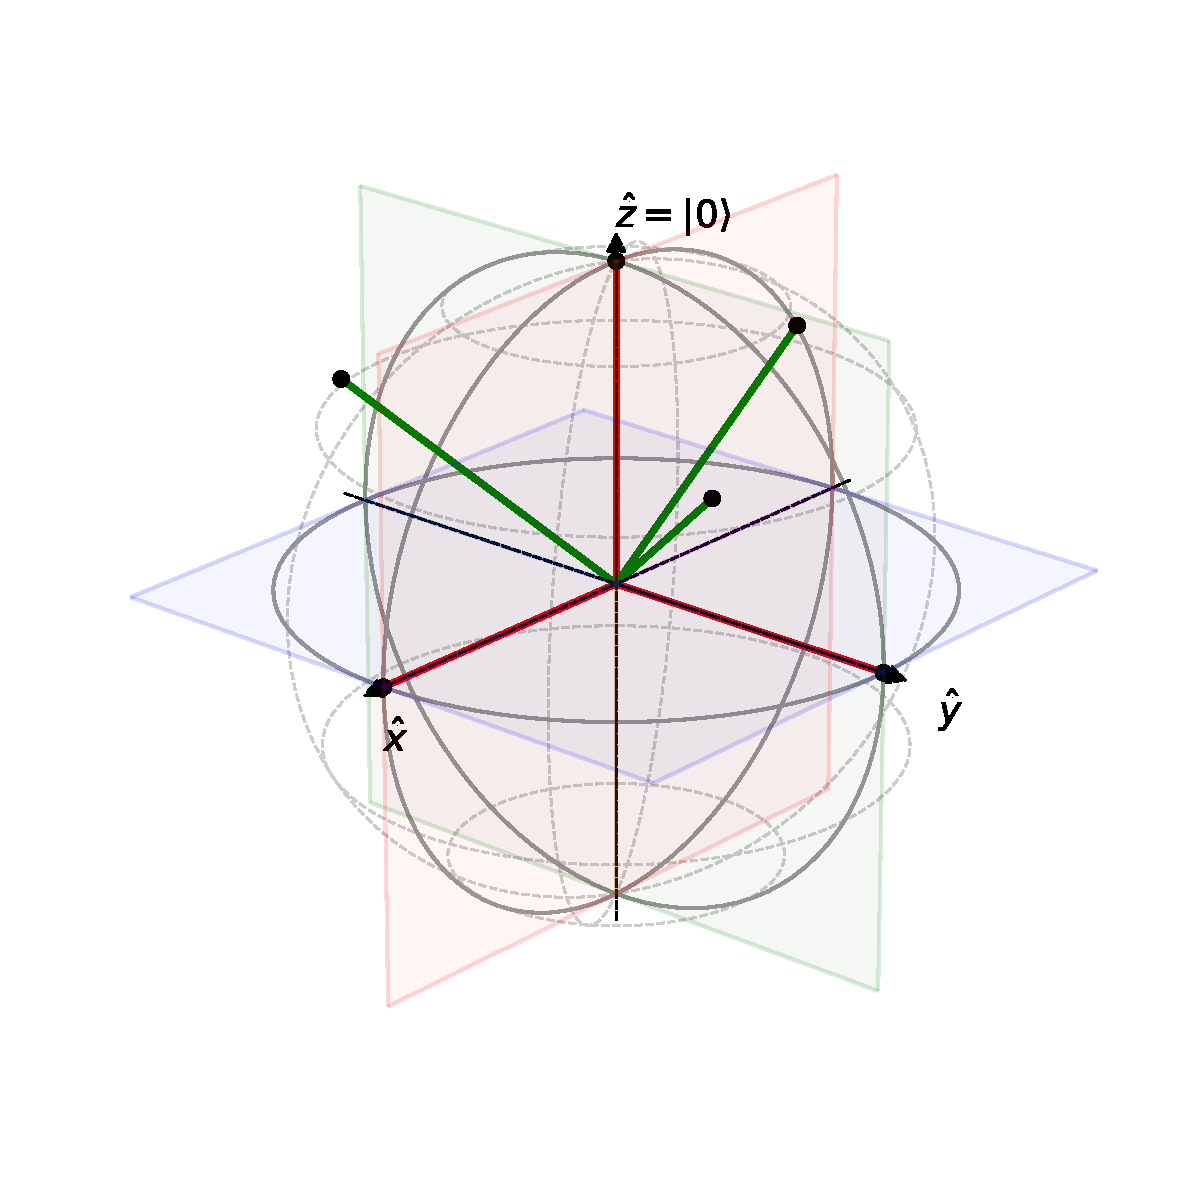
\includegraphics[scale=0.48]{./images/4_1_result.pdf}
  \caption{\label{4_1_vqa} Rotation of initial states. The red represent the initial quantum states, while the green represent the final quantum states.}
\end{figure}

\subsubsection{More usage}
In \MindQuantum, except these two basic usages, \getexpectationwithgrad offers a broader range of application scenarios. The definition of equation that we actually calculate gradient is:
\begin{equation}
  E = \left<\varphi\right|U_l^\dagger H U_r \left|\psi\right>.
\end{equation}
You can set $U_l$ to an empty circuit and $H$ to identity \QubitOperator, so that you can get the projection of the new state on $\ket{\varphi}$ and you can also set $\ket{\varphi}=\ket{\psi}$, $U_l = U_r$ and $H$ to a density matrix, such as $H = \ket{0}\bra{0}$, and the result will be
\begin{equation}
  E=\left|\bra{0}U_r\ket{\psi}\right|^2.
\end{equation}
You can also set the observable to a list of Hamiltonian, so that \MindQuantum\ can calculate the expectation and gradient in parallel.
